\documentclass{beamer}
\usetheme{Boadilla}
\makeatletter
\def\th@mystyle{%
    \normalfont % body font
    \setbeamercolor{block title example}{bg=orange,fg=white}
    \setbeamercolor{block body example}{bg=orange!20,fg=black}
    \def\inserttheoremblockenv{exampleblock}
  }
\makeatother
\theoremstyle{mystyle}
\newtheorem*{remark}{Remark}
\newtheorem*{task}{Task}
\newtheorem*{idea}{Idea:}
\newtheorem*{dood}{}
\usepackage{bbm}
\usepackage{tikz-cd,mathtools}

\newcommand{\A}{\mathbb{A}}
\newcommand{\N}{\mathbb{N}}
\newcommand{\Z}{\mathbb{Z}}
\newcommand{\Q}{\mathbb{Q}}
\newcommand{\R}{\mathbb{R}}
\newcommand{\C}{\mathbb{C}}
\newcommand{\f}{\mathfrak{f}}
\newcommand{\F}{\mathbb{F}}
\newcommand{\g}{\mathfrak{g}}
\newcommand{\K}{\mathbb{K}}
\renewcommand{\l}{\mathfrak{l}}
\newcommand{\p}{\mathfrak{p}}
\renewcommand{\P}{\mathfrak{P}}
\newcommand{\PP}{\mathbb{P}}
\mode<presentation>{}
\usepackage{amscd}
\tikzcdset{ampersand replacement=\&}
\usepackage{tikz-cd}
\tikzcdset{ampersand replacement=\&}
\usepackage{tikz}
\usepackage{mathtools}
\usepackage{array}
\usepackage[utf8]{inputenc}
\usepackage[T1]{fontenc}
\usepackage{textcomp}
\usepackage[english]{babel}
\usepackage{amsmath, amssymb}
\usepackage[mathscr]{euscript}
\usepackage{subcaption}
\usepackage{graphicx}
\usepackage{listings}
\usepackage{xcolor}
\graphicspath{ {./} }
\begin{document}
\title{A Benchmark for Interpretability Methods in DNNs}
\subtitle{(Google Brain)}
\author{Sam Laing }
\institute{University of Tuebingen}
\date{\today}
\begin{frame}
\titlepage
\end{frame}
\begin{frame}
	\frametitle{A Bit of Background}
	\begin{itemize}
		\item Which features in my input are most affecting the model's output?\pause
		\item Deep image classification: "features" = pixels .\pause
		\item Ensembling also possible \pause
		\item Goal: help the engineer understand how their model is performing ... \pause 
		\item Austensibly. But are they even right?
	\end{itemize}
\end{frame}
\begin{frame}
	\frametitle{Some of the included interpretability methods}

	* make individual slides and add pictures*
\begin{itemize}
	\item Gradients (sensitivity heatmaps). i.e literally considering the gradient of output wrt. input at each pixel value.  $e = \partial_{x_i} A_n^{\ell} $

\item Guided Backprop (sort of a tidied up sensitivity map by only looking at positive values)
\item Integrated Gradient: for each pixel, compare to baseline $x^0$ (often elected to be black pixel)  \\

	%\[
	%	e = \frac{(x_i - x_i^0)}{k} \sum_{j=1}^{k} {\partial_{x_i} f_w(x^0 + \frac{i}{k}(x-x^0))}
%	\]
\item \underline{Ensembling}: Effectively injecting inputs with Gaussian noise $J$ times and considering mean/variance. Then apply a gradient method. $\eta_i \sim N(\mu , \sigma )$
\item SmoothGrad (SG) $e = \sum_{i=1}^{J} {f( x + \eta_i, A_n^{\ell}) }$
\item SmoothGrad Squared (SG-SQ) $e = \sum_{i=1}^{J} {f( x + \eta_i, A_n^{\ell})^{2} }$
\item VarGrad (VAR) $e = \text{Var}\left(  \sum_{i}^{J} {f(x + \eta_i, A_n^{\ell})}\right) $
\end{itemize}
Notice the similarity between SG-SQ and VarGrad
\end{frame}
\begin{frame}
	\frametitle{Motivation}
	\begin{itemize}
		\item How do we know how well a feature an interpretability method is really perfomative? \pause
		\item Different methods may consider different features important \pause
		\item How can I really say that interpretability method A has chosen better features than interpretabiilty method B?
		\item If only there was a benchmarking framework to do this...
	\end{itemize}
\end{frame}
\begin{frame}
	\frametitle{ROAR (RemOve And Retrain)}
	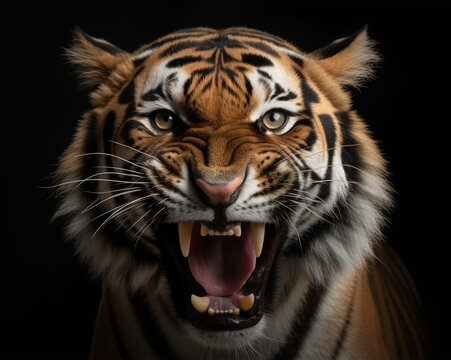
\includegraphics[height=8cm, width=10cm]{tiger.png}
\end{frame}
\begin{frame}
	\frametitle{The idea behind ROAR}
	\begin{itemize}
		\item For each method being considered, sort the feature (pixels) in order of ranked importance by the interpretability method. \\ Creating an ordered tuple $(e_j)_{j=1}^{D}$ of pixel coordinates for each image in the training dataset.
		\item for $j \in \{0, 10, \ldots,100\} $, we replace the top j percent of ranked pixels with the per channel mean of the image for every image and then retrain.
		\item Consider the affect of having dropped the "most informative pixels" as determined by each interpretability.
		\item Investigate how much their removal from the training process effects accuracy.		\item Also a no-retraining variant


	\end{itemize}
\end{frame}

\begin{frame}
	\frametitle{To Retrain Or not To Retrain}
	\begin{itemize}
	\item Without retraining the model, train and test come from different distributions... violates key assumption of ML
	\item Paper therefore argues it is necessary
	\end{itemize}
	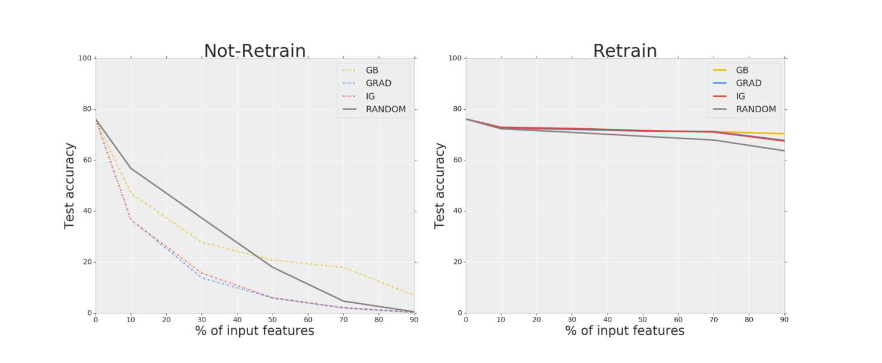
\includegraphics[width=12cm, height=5cm]{retrain_vs_not.png}
\end{frame}
\begin{frame}
	\frametitle{ROAR in Action}
	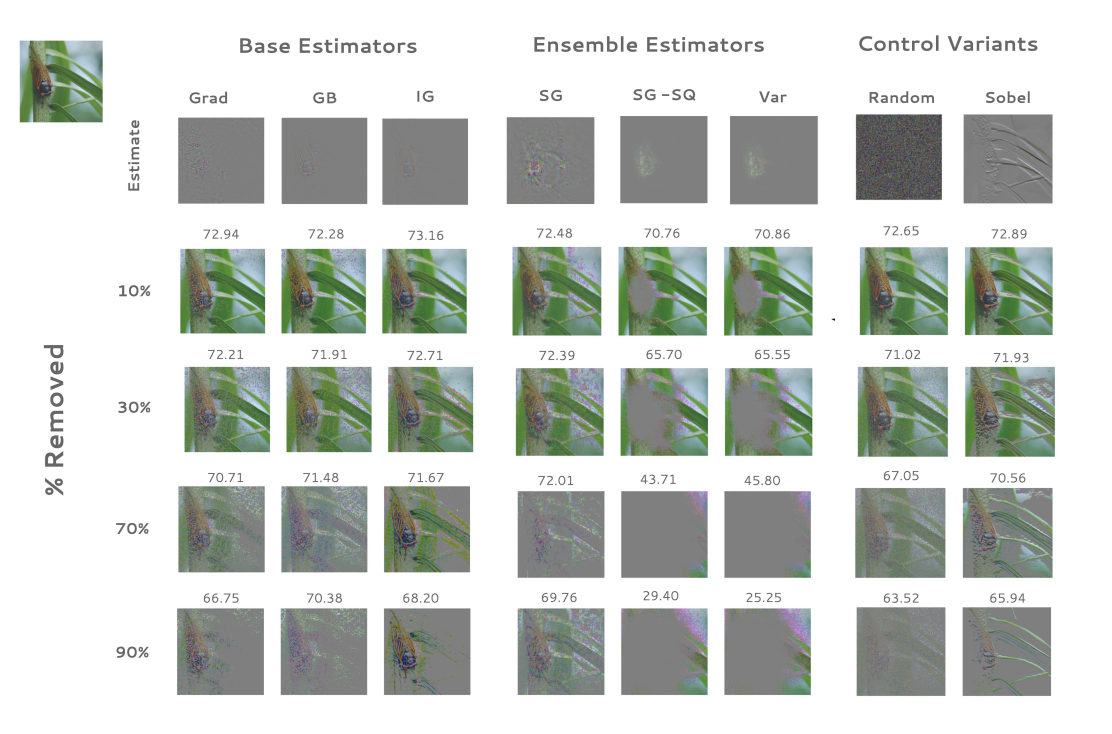
\includegraphics[height=8cm, width=10cm]{ROAR_methods.png}
\end{frame}
\begin{frame}
	\frametitle{An Outline of the Experiment}
	Really just a refinement of above.
	\begin{itemize}
		\item Experiment was performed using a ResNet50 classifier on Imagenet, Birdsnap and Food 101\pause
		\item Along with a number of different interpretability methods, a random ranking was also included: This tells us if the method outperforms random.\pause
		\item  New train and test sets are generated for each $j \in \{0,10,30,50,70,90\} $\pause
		\item For fairness, the model is retrained 5 times for each method (DNN training is noisy) \pause
	\end{itemize}
\end{frame}

\begin{frame}
	\frametitle{Results}
	\begin{itemize}
		\item Surprisingly, replacing large numbers of pixels doesn't remove that much predictive power! \pause
		\item For ImageNet, after 90\% of the pixels are randomly removed, still 63.53\% accuracy relative to the original 78.68\% \pause
		\item Don't worry... this paper is from 2018, they don't stink at training networks :)\pause
		\item According to the paper, SG-SQ and VarGrad are the real heros \pause
	\end{itemize} 
	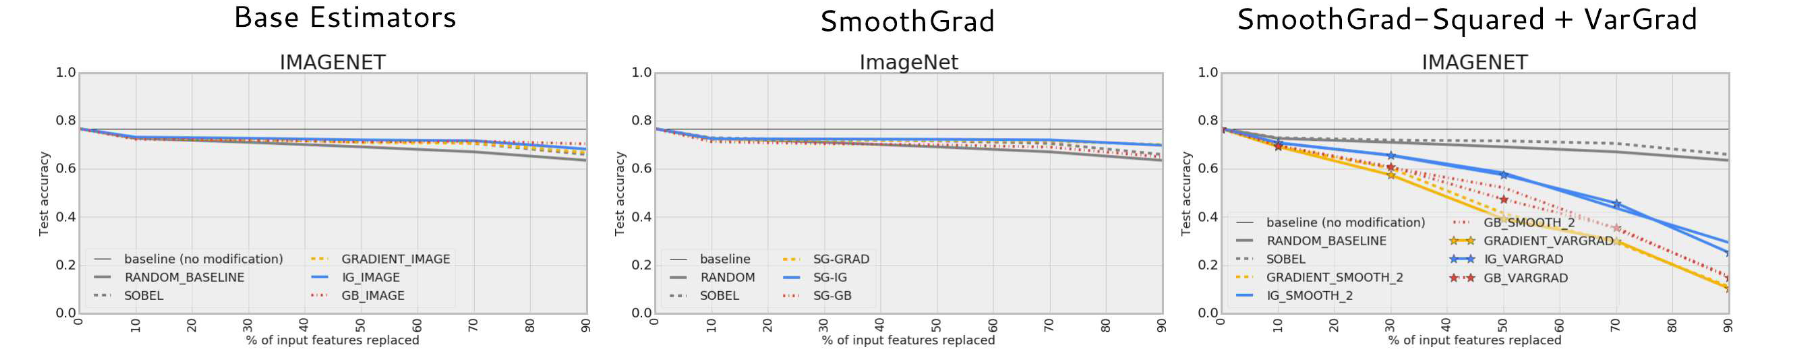
\includegraphics[width=11cm, height=4cm]{ImgNetSG.png}

\end{frame}
\begin{frame}
	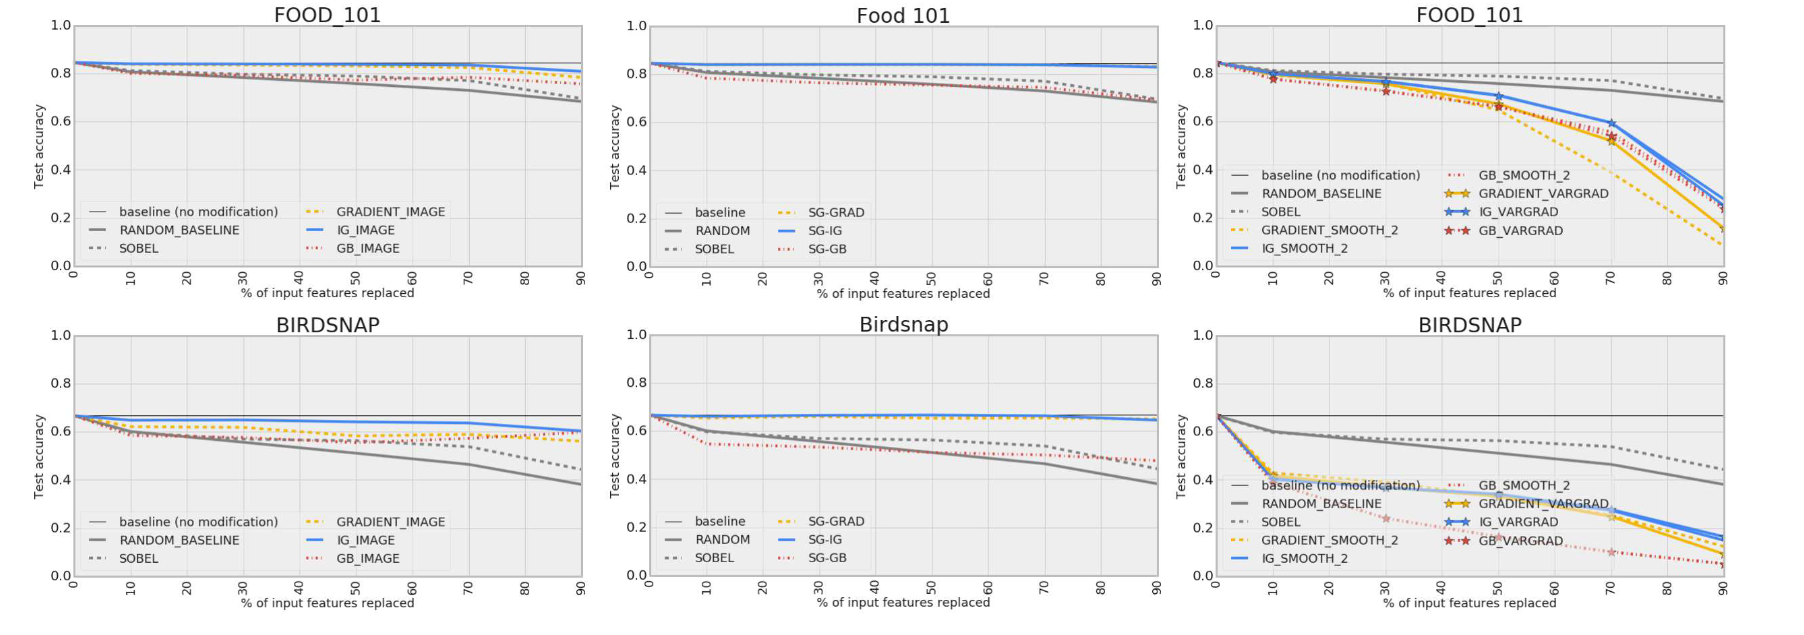
\includegraphics[width=11cm, height=8cm]{other2SG.png}
\end{frame}
\begin{frame}
	\frametitle{Results (cont.)}
	\begin{itemize}
	\item The dataset affects which 
	\end{itemize}
\end{frame}
\begin{frame}
    \frametitle{A Few Possible Issues in the Approach}
    \begin{itemize}
        \item This experiment replaces the top j pixels with the mean of the image.
        \item Is this really the best way?
        \item The mean still conveys possibly useful information
        \item Alternative methods are sometimes advised but most have their own issues.
    \end{itemize}
    \begin{minipage}{0.48\textwidth}
        \centering
        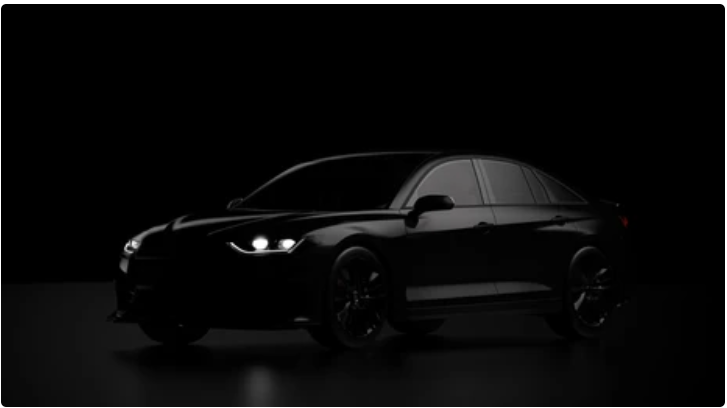
\includegraphics[width=\textwidth, height=3.5cm]{black_car.png}
    \end{minipage}
    \hfill
    \begin{minipage}{0.48\textwidth}
        \centering
        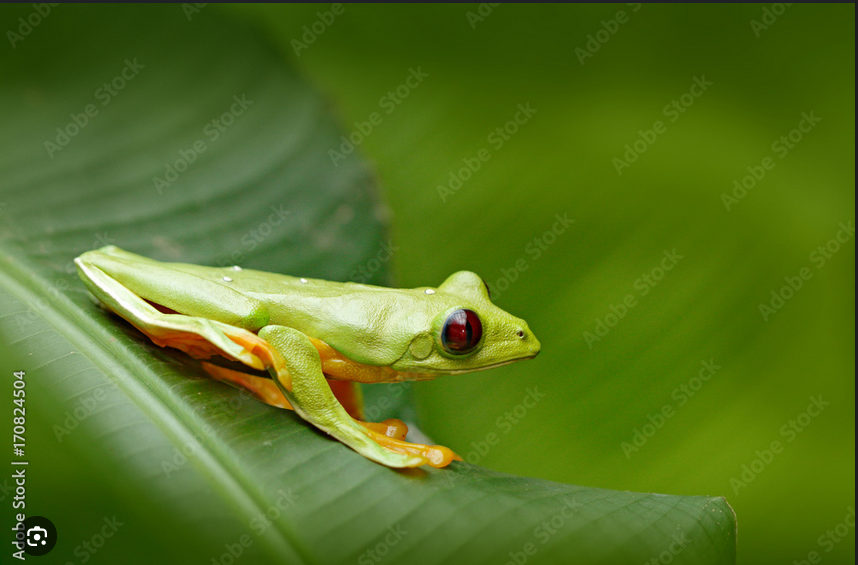
\includegraphics[width=\textwidth, height=3.5cm]{green_frog.png}
    \end{minipage}
\end{frame}
\begin{frame}
	\frametitle{Another possible Issue}
	\begin{itemize}
	\item In practice retraining a large image classifier several times is pretty unfeasible computationally speaking.  (ImageNet with ResNet50 can take 
	\item Without retraining, you run into theoretical violations of ML!
	\end{itemize}
\end{frame}A
\begin{frame}
	\frametitle{Yet Another Possible Issue}

\end{frame}
\begin{frame}
	\frametitle{Why I chose this paper}
\end{frame}
\begin{frame}
	\frametitle{Questions?}
\end{frame}
\end{document}

